\documentclass{ximera}

% add paths to activities with images here
\graphicspath{
{./}
{basic-features/}
}



\newcommand{\RR}{\mathbb R}
\newcommand{\NN}{\mathbb N}
\newcommand{\ZZ}{\mathbb Z}


\DeclareMathOperator{\arcsec}{arcsec}
\DeclareMathOperator{\arccot}{arccot}
\DeclareMathOperator{\arccsc}{arccsc}


\outcome{Familiarization with basic environments and commands in Ximera}

\title{Basic features of Ximera document class}

\begin{document}

\begin{abstract}
Abstract goes here.
\end{abstract}

\maketitle

\subsection*{Structure}

To make a Ximera course, follow directory structure of the current course - \link[https://github.com/XimeraStevens/course-template]{https://github.com/XimeraStevens/course-template}.
Put each activity and all supporting documents into a separate folder.

\subsection*{Environments}

The following environments are available:
{\sf
algorithm,
axiom,
claim,
conclusion,
condition,
conjecture,
corollary,
criterion,
definition,
example,
explanation,
fact,
idea,
lemma,
model,
notation,
observation,
paradox,
procedure,
proposition,
remark,
summary,
template,
theorem,
warning
}.

So you can write, for example, theorems as usual:


\begin{theorem}\label{th1}
Some statements here.
\end{theorem}



Besides that, there are {\it question} environments:
{\sf
problem,
exercise,
question,
exploration,
gradarius
}.
There is no difference between these environments except for title.
Inside these environments you should put interactive elements like
{\sf
multipleChoice,
selectAll,
hint,
feedback,
answer,
grdcell
}.

\subsection*{Basic interactive elements}

Example for {\sf answer} command:

\begin{problem}
The value of $\sin \frac{\pi}{3}$ is equal to $\answer[label=answer:sin]{ \frac{\sqrt{3}}{2} }$, and the value of $\cos \frac{\pi}{3}$ is equal to $\answer[label=answer:cos]{\frac{1}{2}}$.
\end{problem}

You can use {\sf hint} environment to provide hints, and {\sf feedback} environment to provide some message when an attempt to answer is made.

\begin{problem}
$\frac{d}{dx} \sin x$ is equal to $\answer[label=answer:der]{\cos x}$.

\begin{hint}
This is the first hint.
\end{hint}

\begin{hint}
And this is the other one.
\end{hint}

\begin{feedback}
Congrats, you made an attempt to answer this question.
\end{feedback}

\end{problem}

Do not forget to set {\sf label} parameter for {\sf answer} command and for {\sf multipleChoice} and {\sf selectAll} environments.
That is the way to identify these interactive elements and students' answers for these elements. 

Example for {\sf multipleChoice} environment:

\begin{problem}
The limit $\lim_{x \to 0} \frac{\sin x}{x}$ is equal to

\begin{multipleChoice}[label=mlt:lim1]
\choice{$0$}
\choice[correct]{$1$}
\choice{$2$}
\end{multipleChoice}

And the limit $\lim_{x \to 0} (1+x)^{\frac{1}{x}}$ is equal to
\begin{multipleChoice}[label=mlt:lim2]
\choice{$1$}
\choice{$\frac{\pi}{e}$}
\choice[correct]{$e$}
\choice{$\pi$}
\end{multipleChoice}

\end{problem}


Example for {\sf selectAll} environment:

\begin{problem}
Select all odd numbers below

\begin{selectAll}[label=sall:oddnumbers]
\choice[correct]{1}
\choice{2}
\choice[correct]{3}
\choice{4}
\choice[correct]{5}
\end{selectAll}

\end{problem}


If you want a problem to appear only after another one is done, use nested {\it question} environments:

\begin{problem}
After you write 1 in this box $\answer[label=answer:ex1]{1}$, new question will appear.

\begin{problem}
Write 2 in this box $\answer[label=answer:ex2]{2}$.
\end{problem}

\end{problem}


\subsection*{Labeling}

You can label equations and refer to them inside a single activity.

For example, consider equation

\begin{equation}\label{eq:euler_formula}
e^{i \phi} = \cos \phi + i \sin \phi.
\end{equation}

Equation ($\ref{eq:euler_formula}$) ($\leftarrow$ this link should work) is known as Euler's formula.

You can also make links to Ximera's environments.
So link to theorem \ref{th1} should work.

\subsection*{Links}

For all links use {\sf link} command.
For example, here is the link to \link[our GitHub repo]{https://github.com/XimeraStevens/course-template}.

\subsection*{Images}

Use {\sf png} format for images.
Include images inside  {\sf image} environment with {\sf includegraphics} command:
\begin{image}
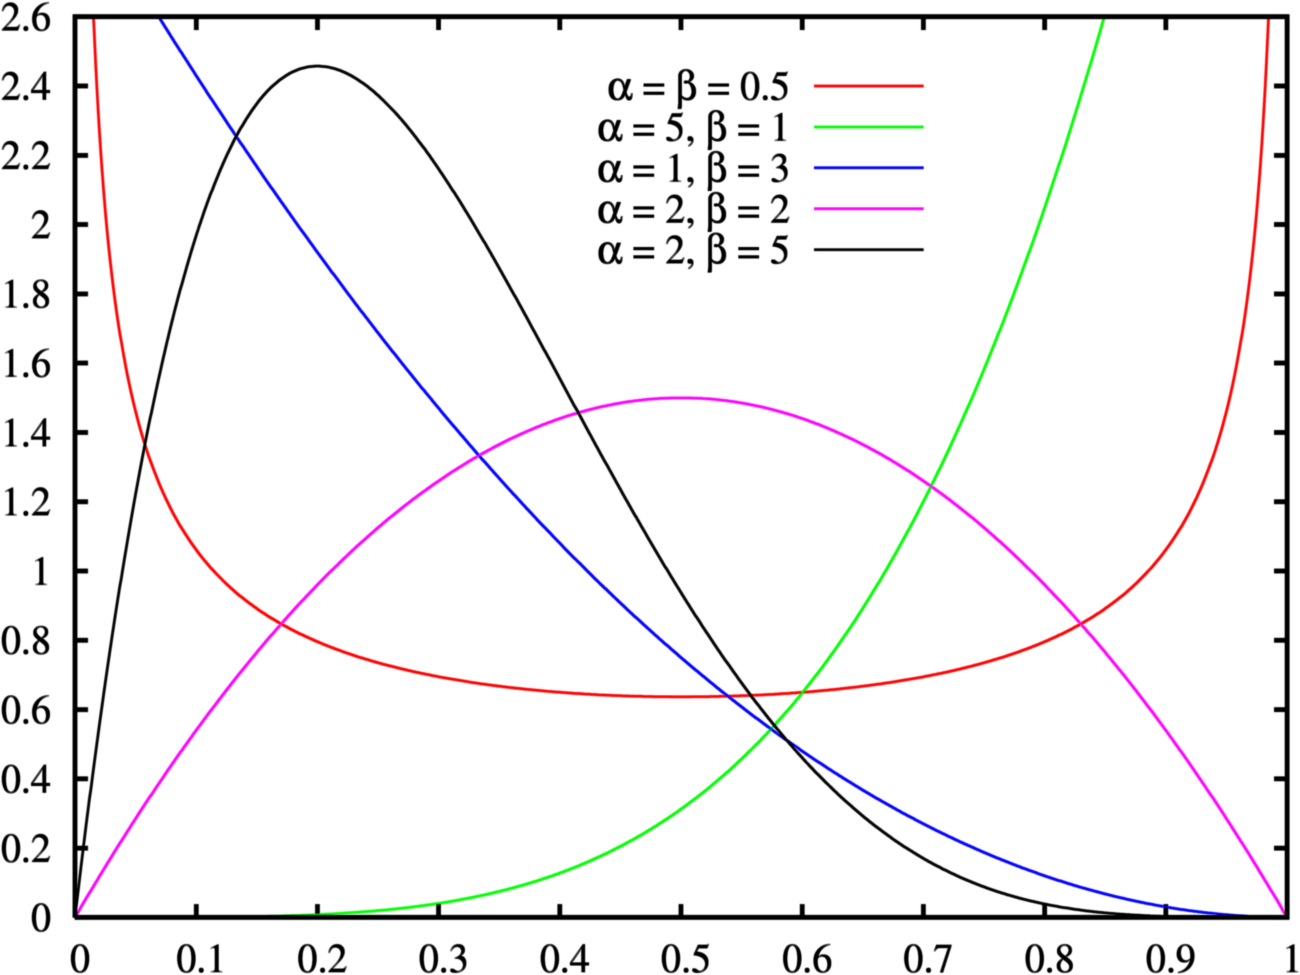
\includegraphics{graphic.png}
\end{image}

\subsection*{Other interactive elements}


You can embed Geogebra widget:

\geogebra{WVGxwKKn}{750}{460}

Do not forget to set its sizes.
Recommended width is 750.

\noindent\rule{12cm}{0.4pt}

YouTube videos: \youtube{gJ1pYz1k0qM}

\noindent\rule{12cm}{0.4pt}

\link[SageMathCells]{https://sagecell.sagemath.org/static/about.html} (example from \link[here]{http://ximera.osu.edu/course/mthomas7/iccalc/first}):

\begin{sageCell}
def Rotate(A,P,theta):
    A1 = [A[0]-P[0],A[1]-P[1]]
    R = [A1[0]*cos(theta)-A1[1]*sin(theta),A1[0]*sin(theta)+A1[1]*cos(theta)]
    return [R[0]+P[0],R[1]+P[1]]
def KochSnowflake(A,B,iterations):
    L = L1 = L2 = L3 = L4 = Graphics()
    P = [(B[0]+2*A[0])/3,(B[1]+2*A[1])/3]
    Q = [(2*B[0]+A[0])/3, (2*B[1]+A[1])/3]
    C = Rotate(A,P,2*pi/3)
    if iterations > 0:
        L1 = L1 + KochSnowflake(A,P,iterations-1)
        L2 = L2 + KochSnowflake(P,C,iterations-1)
        L3 = L3 + KochSnowflake(C,Q,iterations-1)
        L4 = L4 + KochSnowflake(Q,B,iterations-1)
        L = L1 + L2 + L3 + L4
    else:
        L = line([A,P,C,Q,B])
    L.axes(False)
    L.set_aspect_ratio(1)
    return L
@interact
def _(iterations=slider([0..4],label='num iterations',default = 0),size=slider(1,20,label='size',step_size=1, default=9)):
    A=[1,0]
    B=[0,0]
    L = L1 = L2 = L3 = L4 = Graphics()
    P = [(B[0]+2*A[0])/3,(B[1]+2*A[1])/3]
    Q = [(2*B[0]+A[0])/3, (2*B[1]+A[1])/3]
    C = Rotate(A,P,2*pi/3)
    if iterations > 0:
        L1 = L1 + KochSnowflake(A,P,iterations-1)
        L2 = L2 + KochSnowflake(P,C,iterations-1)
        L3 = L3 + KochSnowflake(C,Q,iterations-1)
        L4 = L4 + KochSnowflake(Q,B,iterations-1)
        L = L1 + L2 + L3 + L4
    else:
        L = line([A,P,C,Q,B])
    L.axes(False)
    L.set_aspect_ratio(1)
    L.show(figsize=[size,size])
    
\end{sageCell}















\end{document}
